\chapter{Método Proposto e Objetivo}

A parte operacional da metodologia divide-se em três etapas: 1- Geração de dados sintéticos, 2- Treinamento e 3- Identificação. Cada uma destas etapas será realizada por um programa computacional específico, estes programas vão funcionar de forma independente.

O primeiro programa tem por objetivo gerar dados sintéticos que devem simular os resultados obtidos num levantamento de um perfil composto.
\usetikzlibrary{calc,trees,positioning,arrows,chains,shapes.geometric,%
	decorations.pathreplacing,decorations.pathmorphing,shapes,%
	matrix,shapes.symbols}
\tikzset{
	>=stealth',
	punktchain/.style={
		rectangle, 
		rounded corners, 
		% fill=black!10,
		draw=black, very thick,
		text width=10em, 
		minimum height=3em, 
		text centered, 
		on chain},
	line/.style={draw, thick, <-},
	element/.style={
		tape,
		top color=white,
		bottom color=blue!50!black!60!,
		minimum width=8em,
		draw=blue!40!black!90, very thick,
		text width=10em, 
		minimum height=3.5em, 
		text centered, 
		on chain},
	every join/.style={->, thick,shorten >=1pt},
	decoration={brace},
	tuborg/.style={decorate},
	tubnode/.style={midway, right=2pt},
}

\begin{figure}[H]
\centering
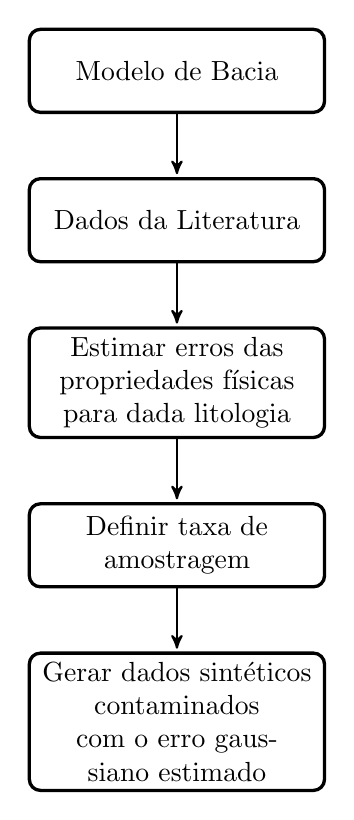
\begin{tikzpicture}
[node distance=.8cm,
start chain=going below,]
\node[punktchain, join]  {Modelo de Bacia};
\node[punktchain, join]   {Dados da Literatura};
\node[punktchain, join]   {Estimar erros das propriedades físicas para dada litologia};
\node[punktchain, join] {Definir taxa de amostragem};
\node[punktchain, join, ] {Gerar dados sintéticos contaminados com o erro gaussiano estimado};

\end{tikzpicture}
\caption{Fluxograma do programa de geração dos dados sintéticos}
\end{figure}


O programa da etapa de Treinamento será alimentado com dados de perfilagens cujas respectivas fácies litológicas são conhecidas (inicialmente serão usados dados sintéticos e posteriormente dados reais). Este programa vai gerar um arquivo com os dados do treinamento, que será usado pelo programa de Operação. Esta é a fase de aprendizagem da rede.


\begin{figure}[H]
	\centering
	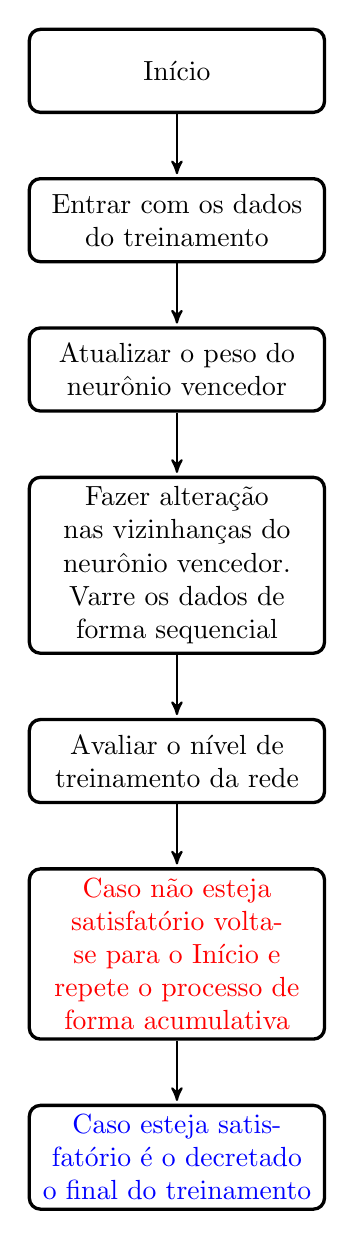
\begin{tikzpicture}
	[node distance=.8cm,
	start chain=going below,]
	\node[punktchain, join]  {Início};
	\node[punktchain, join] (L1)  {Entrar com os dados do treinamento};
	\node[punktchain, join]   {Atualizar o peso do neurônio vencedor};
	\node[punktchain, join] (L2) {Fazer alteração nas vizinhanças do neurônio vencedor. Varre os dados de forma sequencial};
	\node[punktchain, join, ] {Avaliar o nível de treinamento da rede};
	\node[punktchain, join, ] {\color{red}Caso não esteja satisfatório volta-se para o Início e repete o processo de forma acumulativa};
	\node[punktchain, join, ] {\color{blue}Caso esteja satisfatório é o decretado o final do treinamento};	
	\end{tikzpicture}
	\caption{Fluxograma do programa de treinamento da rede neuronal de kohonen.}
\end{figure}

O programa da etapa de identificação vai fazer a classificação, de forma autônoma, das facies litológicas em poços a partir dos dados de perfilagem em poços nos quais a litologia é desconhecida. A aprendizagem da rede deve ocorrer de forma continuada, quanto mais informação temos sobre situações nas quais a litologia é conhecida mais bem preparada estará a rede em termos de aprendizagem. Este conceito de aprendizagem é acumulativo e isso ocorrerá através da atualização do arquivo com os dados de treinamento.

\begin{figure}[H]
	\centering
	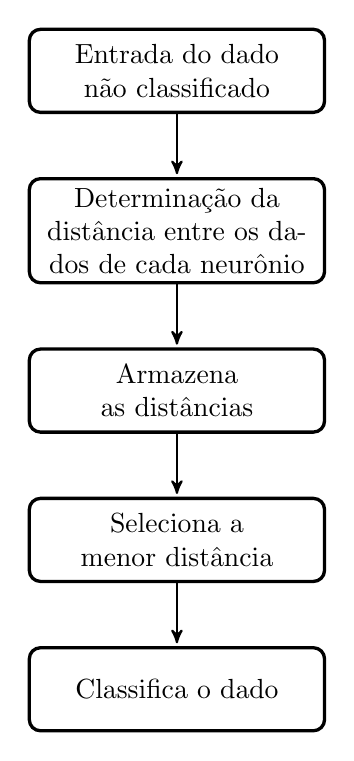
\begin{tikzpicture}
	[node distance=.8cm,
	start chain=going below,]
	\node[punktchain, join]  {Entrada do dado não classificado};
	\node[punktchain, join] (L1)  {Determinação da distância entre os dados de cada neurônio };
	\node[punktchain, join]   {Armazena as distâncias};
	\node[punktchain, join] (L2) {Seleciona a menor distância};
	\node[punktchain, join, ] {Classifica o dado};	
	\end{tikzpicture}
	\caption{Fluxograma do programa de identificação da rede.}
\end{figure}

Durante a elaboração dos programas será necessário testar a usa eficiência. Estes testes serão realizados através de dados sintéticos que serão gerados por um terceiro programa, gerador de dados sintéticos. Este programa será alimentados com informações da literatura. Após os testes com dados sintéticos a metodologia será validada com dados reais, posteriormente depois de cumpridas todas estas etapas, a metodologia estará pronta para ser utilizada em situações reais.

É importante salientar que neste método o conhecimento do funcional geofísico, que rege a relação entre litologia e as propriedades físicas das rochas, não é necessário durante o processo. O conceito de inteligência artificial que será utilizado prescinde do funcional geofísico, o aprendizado é feito através da identificação de padrões recorrentes, sendo este ponto positivo na metodologia, pois o funcional geofísico, que por vezes é desconhecido ou de alta complexidade, exige uma modelagem matemática custosa.

O ponto negativo é a necessidade de se ter muitos dados já analisados em situações conhecidas e variadas para a realização da etapa de treinamento. A etapa de treinamento tem um custo computacional alto.

%\begin{center}
%\smartdiagram[flow diagram:vertical]{Modelo, Dados da literatura, Erro, Taxa de amostragem, Dado sintéticos}
%\end{center}



\section{Objetivo}
O principal objetivo deste projeto é desenvolver um programa computacional do tipo “ machine learning ”, que será implementado na forma de uma Rede Neuronal Artificial (RNA) dentro do contexto da inteligência artificial. Este programa deve ter a capacidade de identificar, de forma autônoma, fácies litológicas a partir de dados de perfilagem de poços sem a necessidade do uso de um funcional geofísico.

É importante salientar que a metodologia que será desenvolvida neste projeto tem aplicação direta tanto na indústria de exploração mineral, quanto na de água, e na de petróleo e gás.
